% !TEX TS-program = pdflatex
% !TEX encoding = UTF-8 Unicode

\documentclass{beamer}
% for handouts: \documentclass[handout]{beamer}

%\setbeamertemplate{background canvas}[vertical shading][bottom=white,top=structure.fg!25]
% or whatever

\usetheme[compress]{Amsterdam}
%\setbeamertemplate{headline}{}
%\setbeamertemplate{footline}{}
%\setbeamersize{text margin left=0.5cm}
  
\usepackage[english]{babel}
\usepackage{listings}
\usepackage{geometry}
\usepackage{hyperref}
\usepackage{multicol}



\usepackage{color}

\usepackage[utf8]{inputenc}
\usepackage[T1]{fontenc}
\usepackage{lmodern}

\lstset{
basicstyle=\scriptsize\ttfamily,
columns=flexible,
breaklines=true,
numbers=left,
%stepsize=1,
numberstyle=\tiny,
backgroundcolor=\color[rgb]{0.85,0.90,1}
}


\begin{document}

\title[Automated Content Analysis with Python]{\textbf{Four-day workshop\\ Automated Content Analysis with Python} \\ Day 1}
\author[Damian Trilling]{Damian Trilling \\ ~ \\ \footnotesize{d.c.trilling@uva.nl \\@damian0604} \\ \url{www.damiantrilling.net}}
\date{11--9--2017}
\institute[UvA]{Afdeling Communicatiewetenschap \\Universiteit van Amsterdam}



\begin{frame}{}
\titlepage
\end{frame}





\section{Introducing\ldots}
\subsection{\ldots the people}

\begin{frame}
	Introducing\ldots \\
	~~~~~~~~\ldots the people
\end{frame}

\begin{frame}{Introducing\ldots}
	{\huge{Damian}}
	\small{}
	\begin{columns}
		\column{.3\textwidth}
		\makebox[\columnwidth]{
			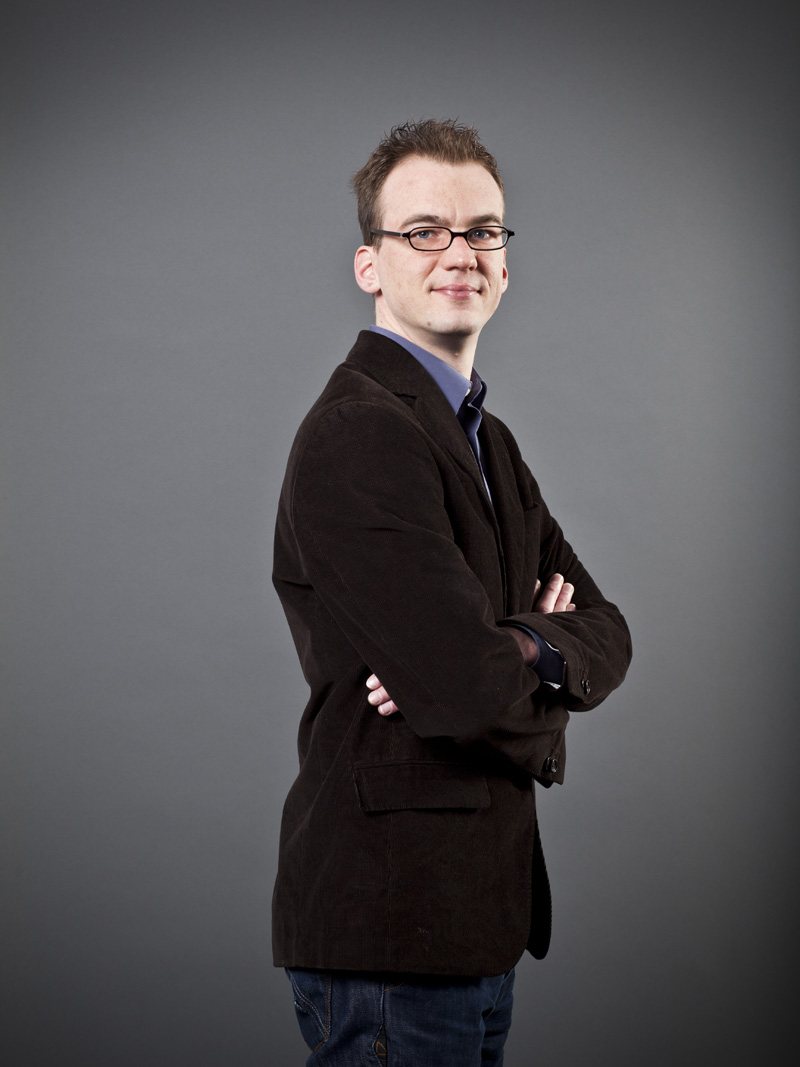
\includegraphics[width=\columnwidth,height=\paperheight,keepaspectratio]{damian.jpg}}
		\column{.7\textwidth}
		dr. Damian Trilling \\
		Assistant Professor Political Communication \& Journalism \\
		\begin{itemize}
			\item studied Communication Science in M\"unster and at the VU 2003--2009
			\item PhD candidate @ ASCoR 2009--2012
			%\item now: Universitair Docent (UD) / Assistant Professor
			\item interested in political communication and journalism in a changing media environment and in innovative (digital, large-scale, computational) research methods
		\end{itemize}
		@damian0604 ~~ d.c.trilling@uva.nl ~~ REC-C~8\textsuperscript{th}~floor ~~ \url{www.damiantrilling.net} 
	\end{columns}
\end{frame}



\begin{frame}{Introducing\ldots}
	{\huge{You}}
	\small{}
	\begin{columns}
		\column{.3\textwidth}
		\makebox[\columnwidth]{
			
\includegraphics[width=\columnwidth,height=\paperheight,keepaspectratio]{mannetje.png}}
		\column{.7\textwidth}
		Your name?\\
		Your background?\\
		Your reason to follow this course?
	\end{columns}
\end{frame}











%
%
%\begin{frame}{Today}
%\tableofcontents
%\end{frame}
%

\section{Today}
\begin{frame}{Today}
	\begin{itemize}
		\item Why Python?
		\item How does Python relate to software you might be familiar with, such as SPSS, STATA, or R?
	\item An introduction to data types – or why a “variable” is not what you might think
	\item Structure of a program
	\item Loops \& conditions
	\item Handling files
	\item \textbf{Play around!}
	\end{itemize}
	
\end{frame}





\section{Why Python?}
\begin{frame}[plain]
	Why Python?
\end{frame}


\begin{frame}{What is Python?}
	\begin{block}{What?}<1->
		\begin{itemize}
			\item A language, not a specific program
			\item Huge advantage: flexibility, portability
			\item One of \emph{the} languages for data analysis. %\tiny{(The other one is R.)}
			%\onslide<2>{ \\\tiny{But Python is more flexible---the original version of Dropbox was written in Python. I'd say: R for numbers, Python for text and messy stuff. But that's just my personal view.}}
		\end{itemize}
	\end{block}
	
	\begin{block}{Which version?}<3->
		We use Python 3. \\ 
		\footnotesize{\url{http://www.google.com} or \url{http://www.stackexchange.com} still offer a lot of Python2-code, but that can easily be adapted. Most notable difference: In Python 2, you write {\tt print "Hi"}, this has changed to {\tt print ("Hi")}}\\
	\end{block}
\end{frame}



\begin{frame}{Comparing Python to things you are familiar with}
	{\tiny{A slightly un-nuanced list:}}
	\begin{itemize}
		\item SPSS, STATA, and R come from a statistics background, Python from a computer science background \\
	\footnotesize{$\Rightarrow$ In R, things are often thought of as vectors and matrices.} \\
	\footnotesize{$\Rightarrow$ But you don't have to know anything about statistics to work with Python (but you \emph{can} if you want to)}
	   \item SPSS and STATA (and to a lesser extend also R) assume that your data are a \emph{table}, while Python regularly uses other data structures (like \emph{lists} or \emph{dictionaries})
	\item SPSS and STATA are really bad in dealing with \emph{text}
	\item Many things you can do in Python you can also do in R and vice versa	
	\item \emph{Huge} community of people using Python for processing text, and many great packages
	\end{itemize}
\end{frame}



\begin{frame}{If it's not a program, how do you work with it?}
	\begin{block}{Interactive mode}<1->
		\begin{itemize}
			\item Just type {\tt python3} on the command line, and you can start entering Python commands {\tiny{(You can leave again by entering {\tt quit()})}}
			\item Great for quick try-outs, but you cannot even save your code
		\end{itemize}
	\end{block}
	
	\begin{block}{An editor of your choice}<2->
		\begin{itemize}
			\item Write your program in any text editor, save it as {\tt myprog.py}
			\item and run it from the command line with {\tt ./myprog.py} or {\tt python3 myprog.py}
		\end{itemize}
	\end{block}
\end{frame}


\begin{frame}{If it's not a program, how do you start it?}
	\begin{block}{An IDE (Integrated Development Environment)}<1->
		\begin{itemize}
			\item Provides an interface
			\item Both quick interactive try-outs and writing larger programs
			\item We use spyder, which looks a bit like RStudio (and to some extent like Stata)
		\end{itemize}
	\end{block}
	
	
	\begin{block}{Jupyter Notebook}<2->
		\begin{itemize}
			\item Runs in your browser
			\item Stores results and text along with code
			\item Great for \emph{interactive} playing with data and for sharing results
		\end{itemize}
	\end{block}
	
\end{frame}


{\setbeamercolor{background canvas}{bg=black}
	\begin{frame}[plain]
		\makebox[\linewidth]{
			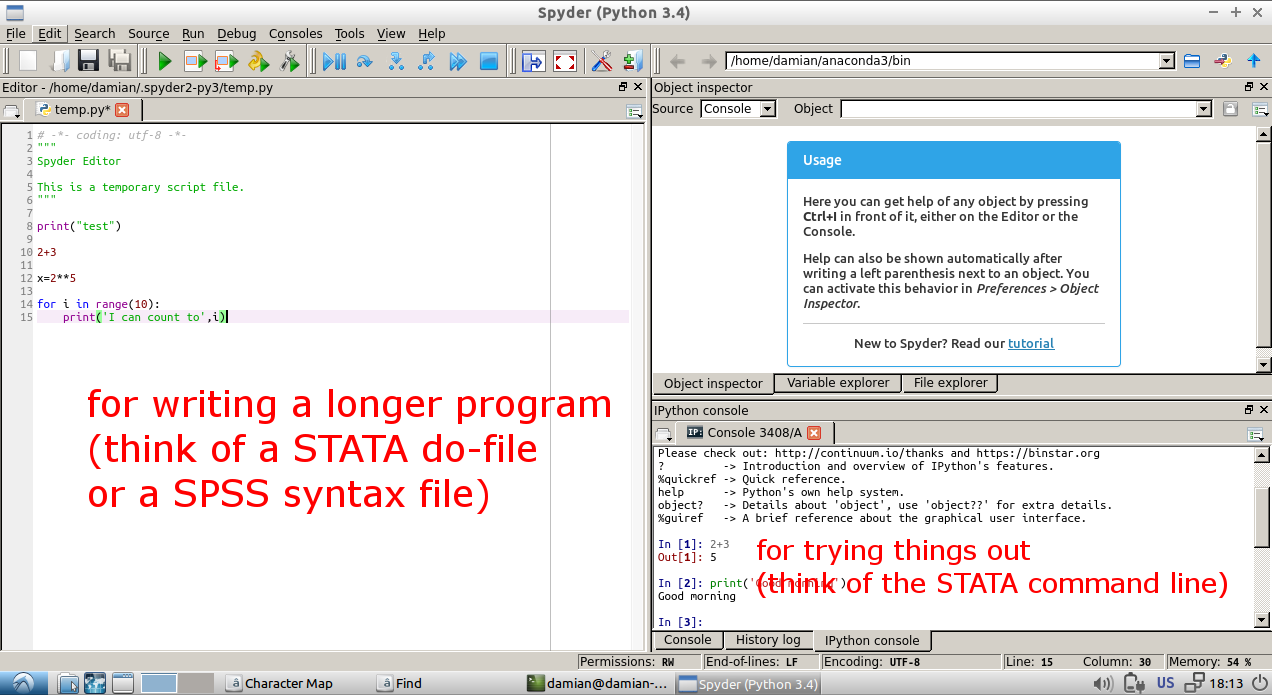
\includegraphics[width=\paperwidth,height=\paperheight,keepaspectratio]{spyder-uitleg.png}
		}
	\end{frame}
	
	\begin{frame}[plain]
		\makebox[\linewidth]{
			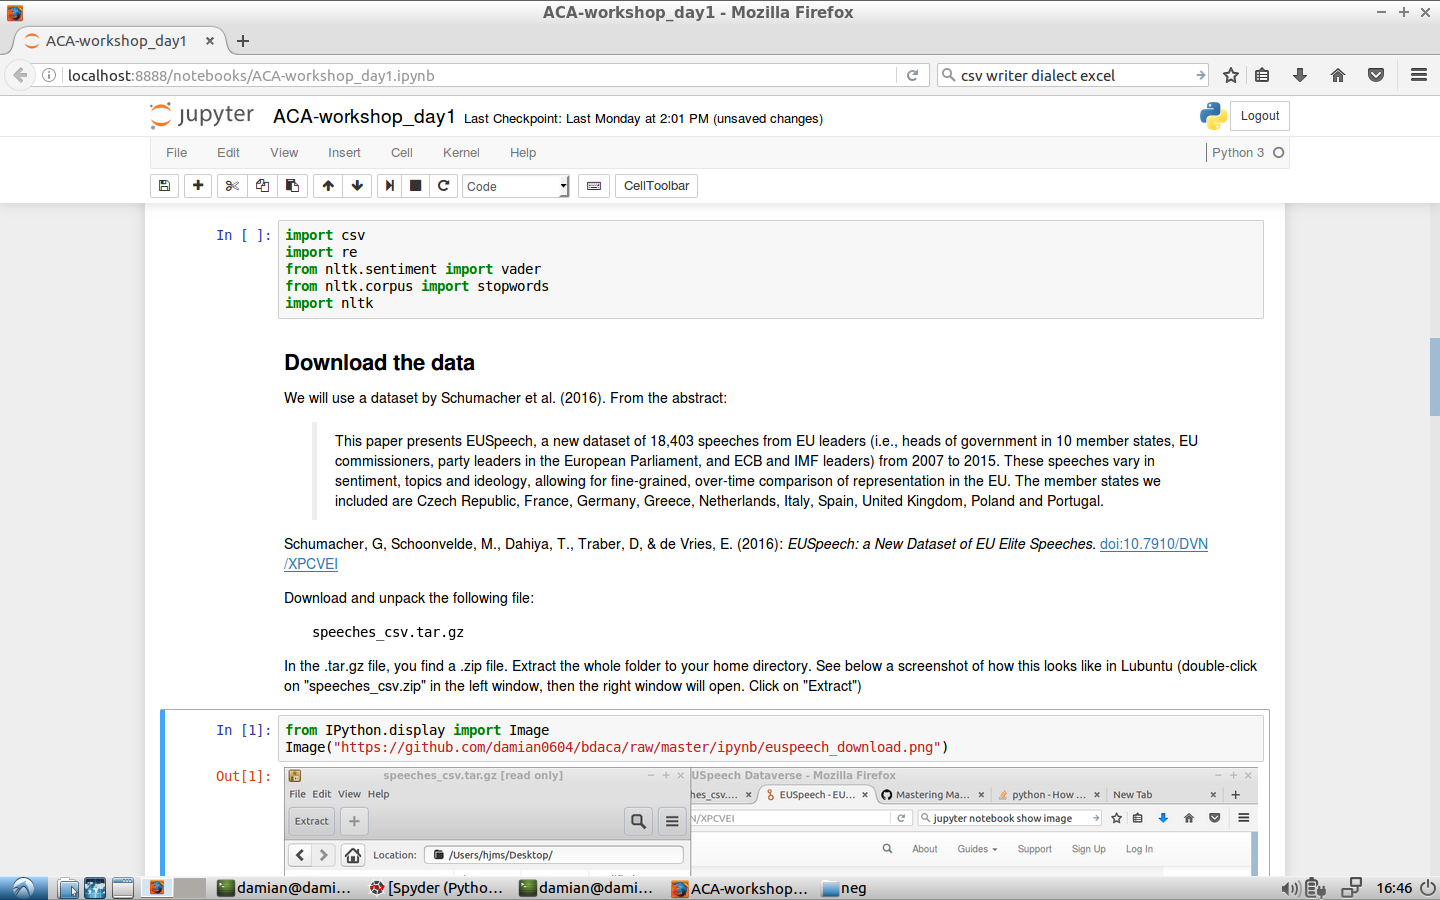
\includegraphics[width=\paperwidth,height=\paperheight,keepaspectratio]{jupyternotebook.png}
		}
	\end{frame}
	
}






\begin{frame}[plain]
	Let's start up a Python environment and write a Hello-world-program!
\end{frame}


\begin{frame}[fragile]{Start playing!}
Exercises 
\vspace{.5cm}
\textbf{1. Run a program that greets you.}\\
The code for this is 
\begin{lstlisting}
print("Hello world")
\end{lstlisting}
After that, do some calculations. You can do that in a similar way:
\begin{lstlisting}
a=2
print(a*3)
\end{lstlisting}
Just play around.

\vspace{.5cm}
\textbf{Additional ressources}\\
Codecademy course on Python
\url{https://www.codecademy.com/learn/python}

\end{frame}







\section[Basics]{The very, very, basics of programming with Python}
\begin{frame}[plain]
\textbf{The very, very, basics of programming}\\
\vspace{1cm}
You can read all this back in Chapter 4.
\end{frame}
\subsection{Datatypes}


\begin{frame}{Python lingo}
\begin{block}{Basic datatypes (variables)}
\begin{description}
\item[{\color{red}int}] \texttt{32}
\item[{\color{red}float}] \texttt{1.75}
\item[{\color{red}bool}] \texttt{True}, \texttt{False}
\item[{\color{red}string}] \texttt{"Damian"}
\onslide<2->{\scriptsize \item[({\color{red}variable name}] \texttt{firstname})}
\end{description}
\end{block}
\onslide<2->{\textbf{"firstname" and firstname is not the same.\\}}
\onslide<3->{\textbf{"5" and 5 is not the same.}\\ But you can transform it: {\tt{int("5")}} will return 5.}\\
\onslide<3->{\textbf{You cannot calculate \texttt{3 * "5"}} {\tiny{Actually, you can. It gives you "555"}}.\\ But you can calculate {\tt{3 * int("5")}}}
\end{frame}



\begin{frame}{Python lingo}
\begin{block}{More advanced datatypes}
\begin{description}
\item[{\color{red}list}]<2-> \texttt{firstnames = $[$'Damian','Lori','Bjoern'$]$ \\ lastnames = $[$'Trilling','Meester','Burscher'$]$}
\item[{\color{red}list}]<3->\texttt{ages = $[$18,22,45,23$]$}
\item[{\color{red}dict}]<4-> \texttt{familynames= \{'Bjoern': 'Burscher', 'Damian': 'Trilling', 'Lori': 'Meester'\} }
\item[{\color{red}dict}]<4-> \texttt{\{'Bjoern': 26, 'Damian': 31, 'Lori': 25\} }

\end{description}
%Note that the elements of a list, the keys of a dict, and the values of a dict can have any datatype! (It should be consistent, though!)
\end{block}
\end{frame}



\begin{frame}{Python lingo}
\begin{block}{Functions}
\begin{description}
\item[{\color{red}functions}]<2-> Take an input and return something else \\ {\tt{int(32.43})} returns the integer 32. \texttt{len("Hello")} returns the integer 5.\\ 
\item[{\color{red}methods}]<3-> are similar to functions, but directly associated with an object. {\tt{"SCREAM".lower()}} returns the string "scream"
\end{description}
\end{block}
\onslide<4->{Both functions and methods end with \texttt{()}. Between the \texttt{()}, \emph{arguments} can (sometimes have to) be supplied.}
\end{frame}


\subsection[Indention]{Indention: The Python way of structuring your program}
\begin{frame}[plain]
Indention: The Python way of structuring your program
\end{frame}


\begin{frame}[fragile]{Indention}
\begin{block}{Structure}
The program is structured by TABs or SPACEs
\end{block}

\end{frame}



{\setbeamercolor{background canvas}{bg=black}
\begin{frame}[plain]
\makebox[\linewidth]{
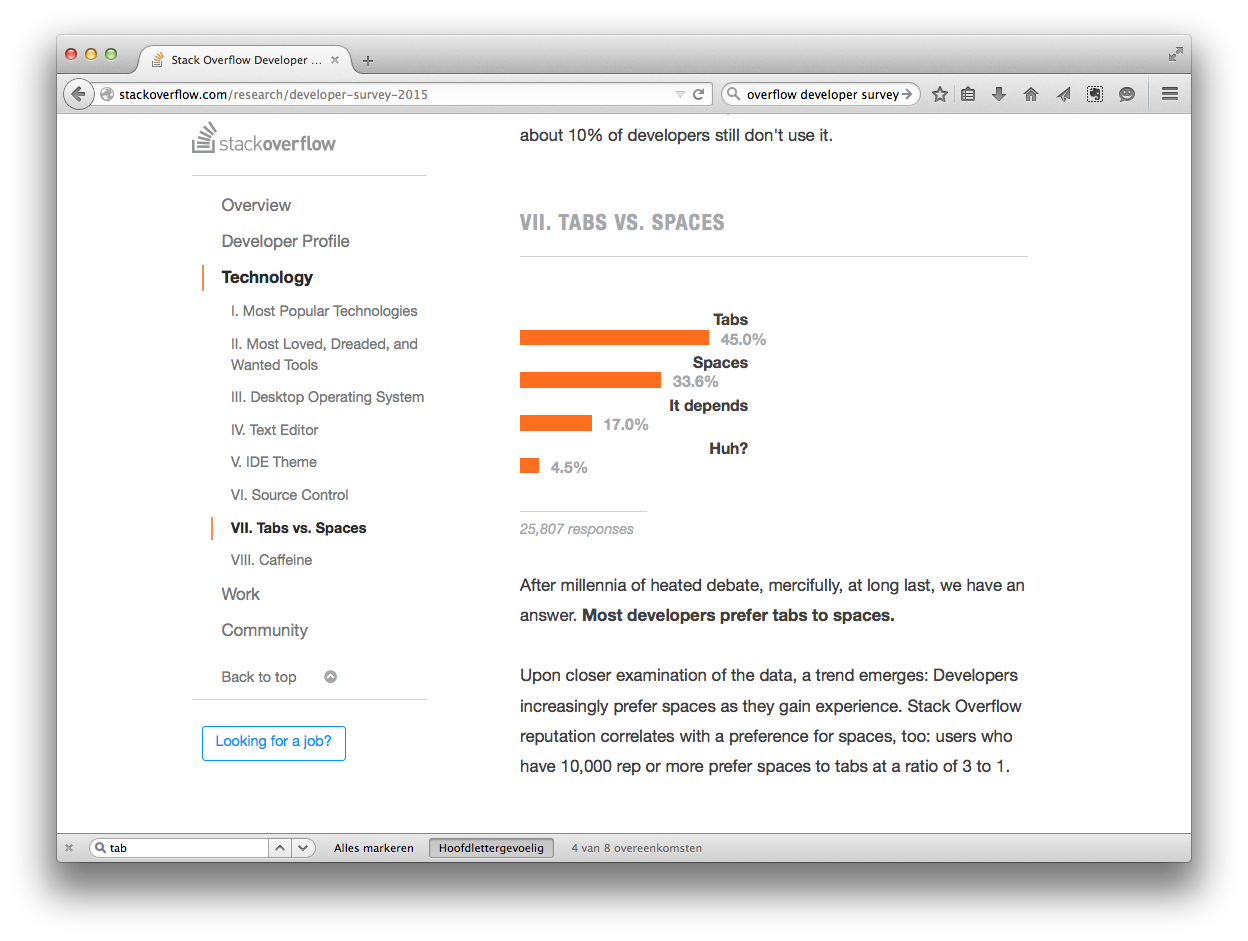
\includegraphics[width=\paperwidth,height=\paperheight,keepaspectratio]{tabsvsspaces}
}
\end{frame}
}

\begin{frame}[fragile]{Indention}
\begin{block}{Structure}
The program is structured by TABs or SPACEs
\end{block}
\begin{lstlisting}
firstnames=['Damian','Lori','Bjoern']
age={'Bjoern': 27, 'Damian': 32, 'Lori': 26}
print ("The names and ages of all BigData people:")
for naam in firstnames:
    print (naam,age[naam])
\end{lstlisting}
\onslide<2->{\textbf{Don't mix up TABs and spaces! Both are valid, but you have to be consequent!!! Best: always use 4 spaces!}}
\end{frame}





\begin{frame}[fragile]{Indention}
\begin{block}{Structure}
The program is structured by TABs or SPACEs
\end{block}
\begin{lstlisting}
print ("The names and ages of all BigData people:")
for naam in firstnames:
    print (naam,age[naam])
    if naam=="Damian":
        print ("He teaches this course")
    elif naam=="Lori":
        print ("She was an assistant last year")
    elif naam=="Bjoern":
        print ("He helps on Wednesdays")
    else:
        print ("No idea who this is")
\end{lstlisting}
\end{frame}


\begin{frame}{Indention}
The line \emph{before} an indented block starts with a \emph{statement} indicating what should be done with the block and ends with a \texttt{:}

\begin{block}{Indention of the block indicates that}<2->
\begin{itemize}
\item<3-> it is to be executed repeatedly (\texttt{for} statement) – e.g., for each element from a list
\item<4-> it is only to be executed under specific conditions (\texttt{if}, \texttt{elif}, and \texttt{else} statements)
\item<5-> an alternative block should be executed if an error occurs (\texttt{try} and \texttt{except} statements)
\item<6-> a file is opened, but should be closed again after the block has been executed (\texttt{with} statement)
\end{itemize}
\end{block}
\end{frame}


\begin{frame}{Let's explore for-loops and the like interactively}
	-- start up a Python interpreter --
\end{frame}



\begin{frame}[plain]
Exercise
\end{frame}




\begin{frame}[fragile]{Exercise}
Write a program that loops over a list of strings and checks whether they contain a substring of your choice.

Things you need:
\begin{itemize}
	\item for loops
	\item if statements
	\item the print() function
	\item the in operator:
\end{itemize}

	
\begin{lstlisting}
In [39]: "a" in "morning"
Out[39]: False

In [40]: "o" in "morning"
Out[40]: True

In [41]: "orn" in "morning"
Out[41]: True
\end{lstlisting}
\end{frame}



\begin{frame}[plain]
	Loading and saving data
\end{frame}


\begin{frame}{Working with files}
\begin{block}{Using pandas}
There is a R-like data structure (a pandas dataframe) in which can directly read CSV, Excel, Stata, \ldots \\
\texttt{
import pandas as pd\\
mydataframe = pd.read\_csv("test.csv")}
\end{block}
But often, we don't necessarily want a \emph{table}. In fact, we might not even want to have the whole file in memory.
\end{frame}



\begin{frame}{Working with files}
	\begin{block}{Reading a file line by line}
\texttt{with open('test.csv') as fi: \\
~~~~for line in fi: \\
~~~~~~~~print(line) \# or do something more useful}
	\end{block}
We thus loop over the file line-by-line, taking one line at a time, do something with it, and take the next one.

This means that we can process files of arbitrary size, as we never have more than one single line in memory. ($\Rightarrow$ very different approach to the concept of "opening" a file than in programs you are familiar with)

\end{frame}



\begin{frame}{Working with files}
	\begin{block}{Writing a file line by line}
		
		\texttt{with open('test.txt',mode='w') as fo: \\
			~~~~fo.writeline('test test test\\n')}
	\end{block}
\texttt{.writeline()} takes a single string as argument,\\ \texttt{.writelines()} a list of strings
	
\end{frame}



\begin{frame}[fragile]{The csv module}
There is a useful package for dealing with csv files. It splits every row in a list of strings (for each column):

\begin{lstlisting}
import csv
name=[]
age=[]
height=[]
with open('/home/damian/mensen.csv') as csvfile:
    reader = csv.reader(csvfile, delimiter=',')
    for row in reader:
        name.append(row[0])
        age.append(row[1])
        height.append(row[2])
print("Done!")
\end{lstlisting}

\end{frame}

\end{document}


